\section{A distributed architecture for IaaS toolkits}

\begin{figure*}
	\centering
	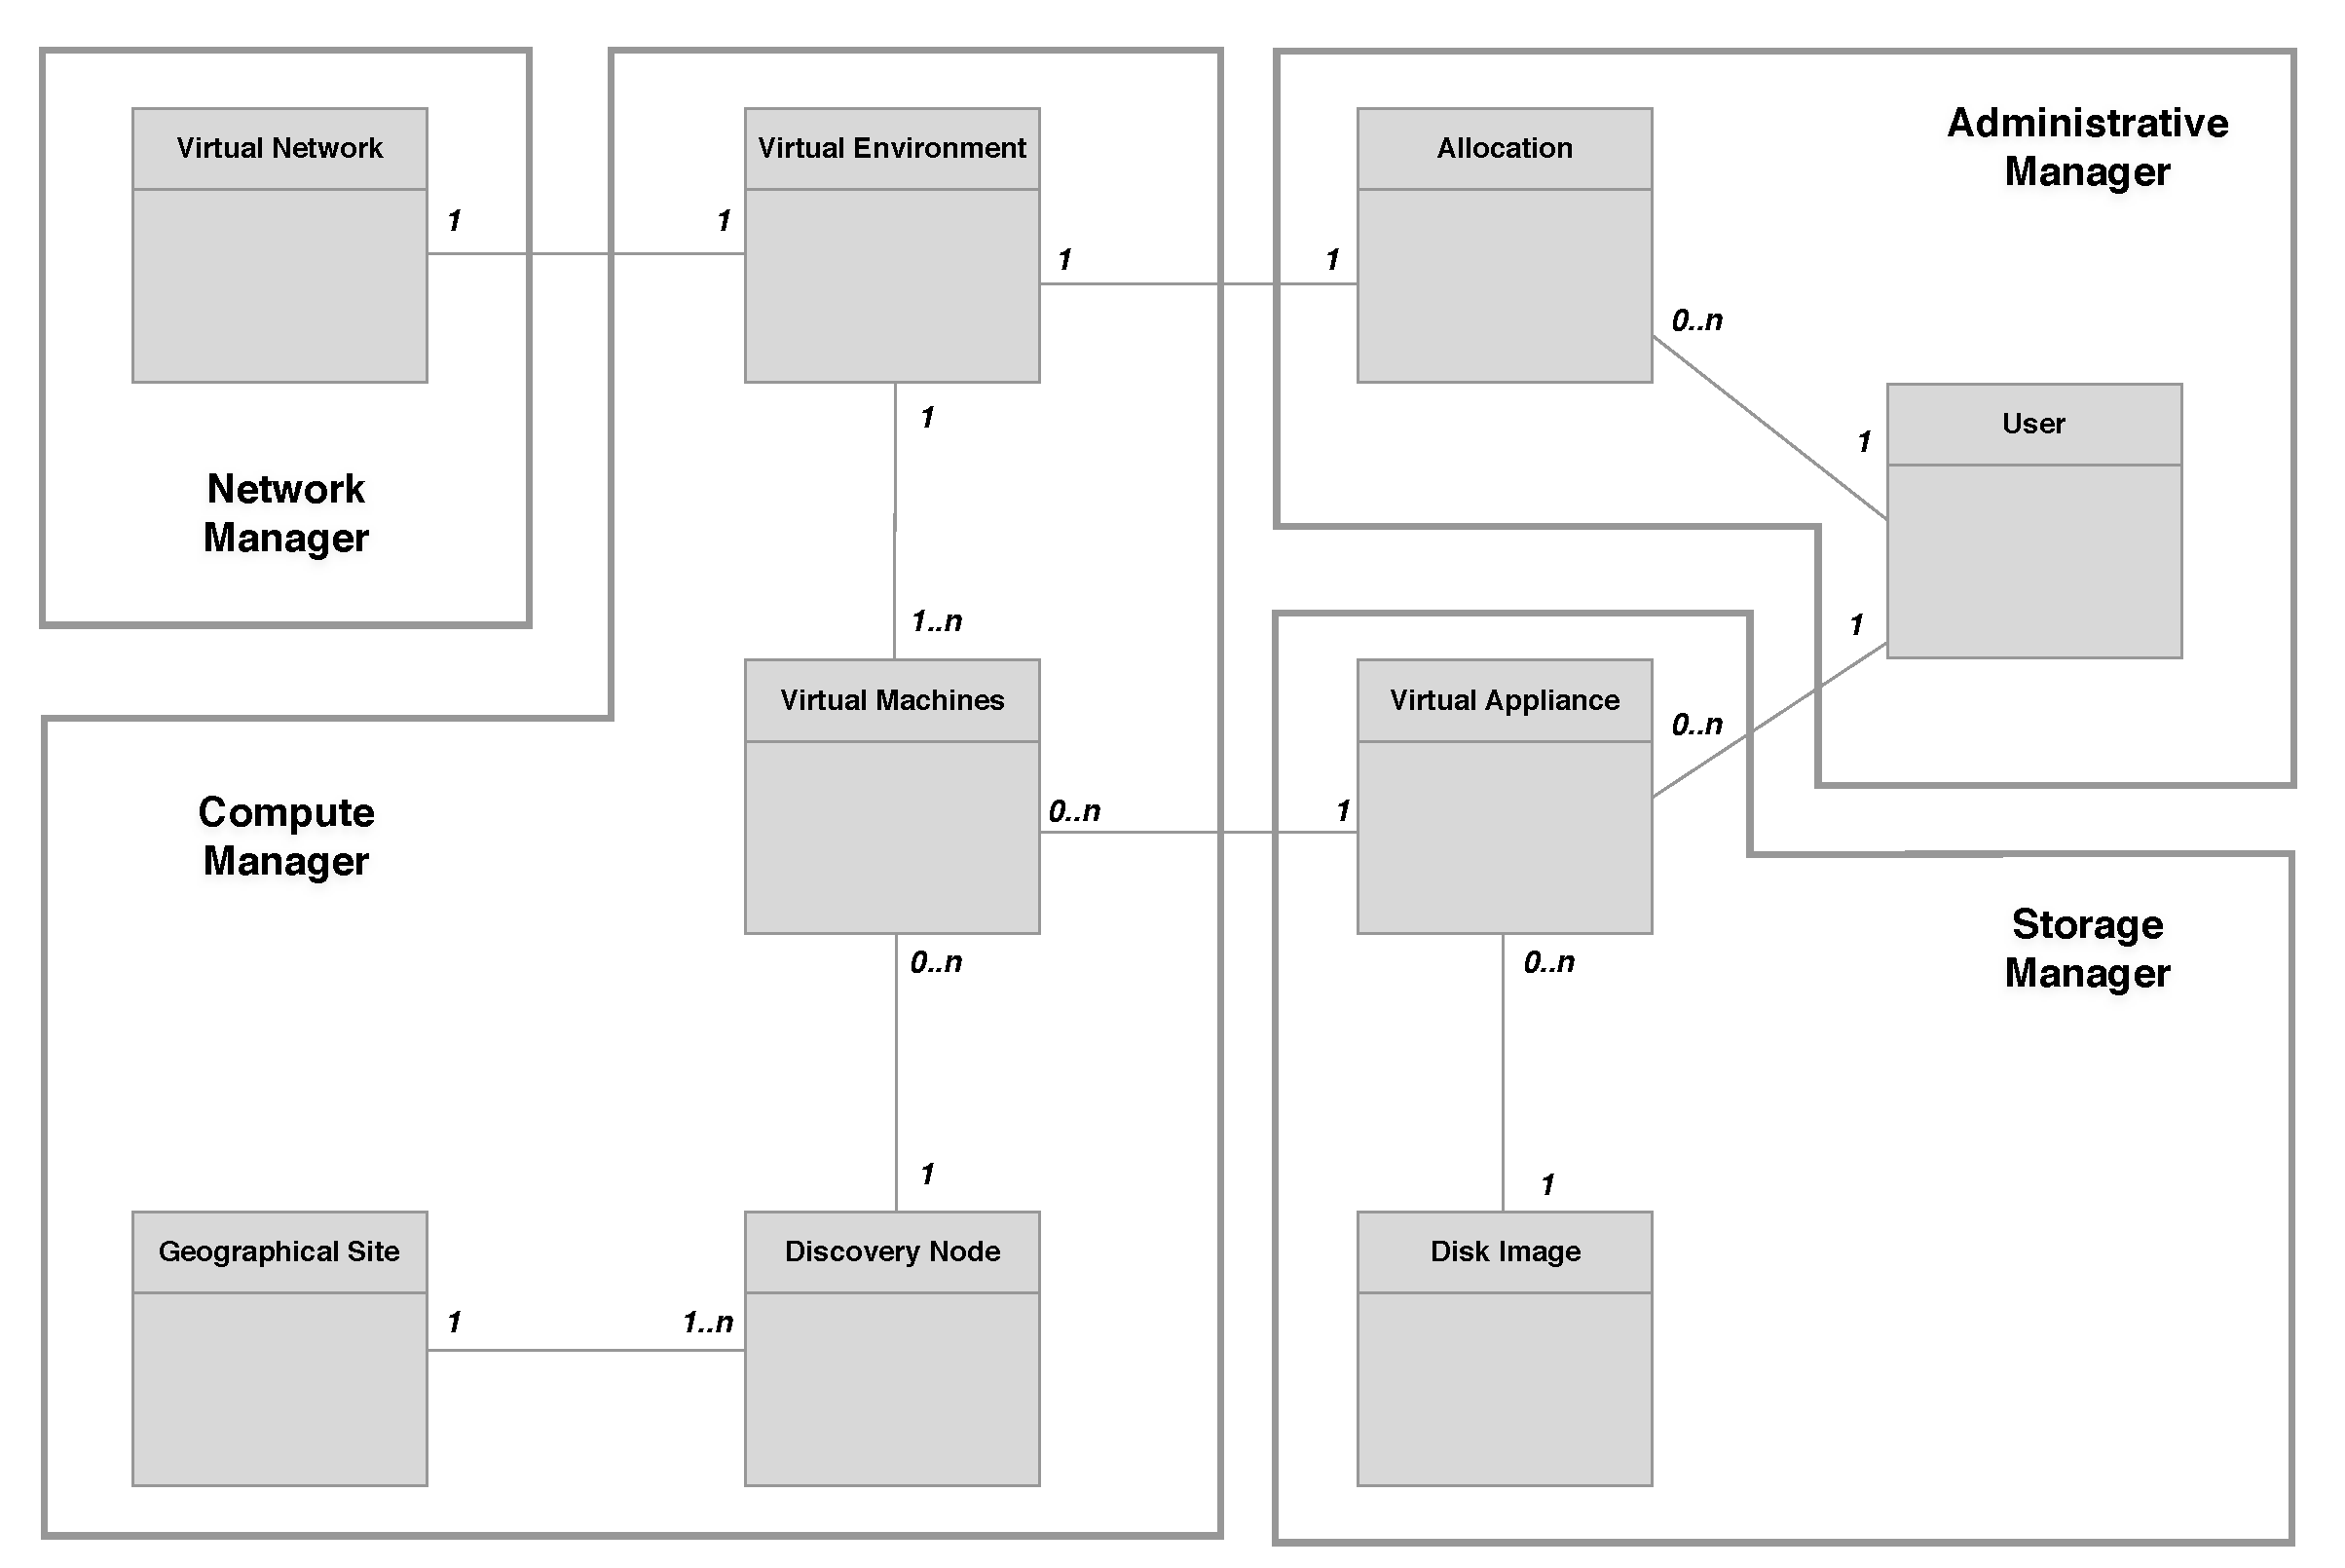
\includegraphics[width=0.91\linewidth]{Figures/mcd_3.pdf}
	\caption{Conceptual schema of the Discovery proposal.}%
	\label{fig:mcd}%
	%\vspace*{-.8cm}
\end{figure*}

In section \ref{cloud_os_concepts} fundamental concepts for the LUC-OS have been
adressed. Leveraging these concepts, we propose a first draft of the LUC-OS
architecture that focus on fundamental services. Each of these services deals 
with one concept from section \ref{cloud_os_concepts} and is described in the 
following listing:

\label{sub:sec:list_services}

\begin{description}

	\item [Compute service] : manages virtual machines' lifecycle.

	\item [Network service] : manages virtual networks.

	\item [Storage service] : manages images and block storage.

	\item [Administrative service] : manages infrastructure and users' permissions.  

\end{description}

In figure \ref{fig:mcd} we propose a conceptual schema that enables an easier 
illustration of data entities with their relationships, that we plan to use in
the LUC-OS. This is a high-level description which aims at defining and 
explaining semantics of our proposal. It is noticeable that this schema is 
partitioned in four block corresponding to the four services previously exposed.

As entities that will be manipulated by services of the LUC-OS are known, an
overview of how entities are involved during virtual machines provisioning can
be given:

\begin{itemize}

	\item A user asks the LUC-OS to provision some computing resources at a 
	specified date:  the \textbf{administrative service} considers the demand 
	and determine  wether it is possible to provide requested resources or not. 
	Once the demand is considered as acceptable, an allocation is created and 
	stored in the  LUC-OS's data structure (a Distributed Hash Table). To enable
	accounting operations such as billing, the allocation will be stored long
	enough.

	\item Once the allocation date has been reached, the \textbf{compute
	service} will ask the ressource scheduler (DVMS) to elect a 
	set of servers that is suitable to spawn the virtual machines, leading to 
	the creation of a new virtual environment which is distributed on the 
	elected servers. \textbf{Network service} then create a new virtual	network
	that is attached to the virtual	environment: during their creations, virtual
	machines will be inter-connected through this virtual network.

	\item The \textbf{storage service} is involved in processes for creating and 
	snapshotting virtual machines. As virtual machine are created from a virtual
	disk image, users will have to specify a virtual appliance (a disk image 
	base flavoured with some pre-installed software). Once a virtual machine is 
	started, it is possible for users to snapshot it: the virtual machine state
	is saved in the distributed data structure.

\end{itemize}